\documentclass[10pt,a4paper]{article}
\usepackage[T1,T2A]{fontenc}
\usepackage[utf8]{inputenc}
\usepackage[russian]{babel}
\usepackage{amssymb}
\usepackage{amsmath}
\usepackage{amsthm}
\usepackage{latexsym}
\usepackage{enumerate}
\usepackage[cm]{fullpage}
\usepackage[pdftex]{graphicx}

\begin{document}

\title{Графы. HW\#2}
\author{Тураев Тимур, 504 (SE)}
\maketitle

\begin{enumerate}
	\item[2.6.] \textit{Пусть у нас имеется улица с односторонним движением, на которой расположено $n$ парковочных мест. На эту улицу последовательно заезжают машины с порядковыми номерами от $1$ до $n$. Каждая $i$-я машина по прибытии едет вначале к своему любимому парковочному месту $f(i)$. Если это место оказывается свободным, то она занимает его. В противном случае она пытается занять первое следующее за ним свободное место. В случае, если такового не оказывается, процесс парковки считается завершившимся неудачей. Функция $f:[n] \rightarrow [n]$ называется парковочной функцией, если задаваемая ею парковка всех $n$ машин прошла успешно.}\\
	\newtheorem*{th0}{Теорема}
	\begin{th0}
	Доказать, что количество всех различных парковочных функций равно $(n+1)^{(n-1)}$
	\end{th0}
	\begin{proof}
	\begin{enumerate}
	\item Слегка поменяем процесс парковки: пусть номера мест идут с нуля и введем еще одно, $n$-е парковочное место, причем оно будет самым обычным: на него можно парковаться; а также введем такое правило: если машина хочет запарковаться на место с номером $n$, которое оказалось занятым, то оно занимает место с номером 1. Если оно занято - то место с номером 2 и т.д. Можно считать, что мы "закольцевали" парковку (или же можем считать, что условие "следующее за ним" мы берем по модулю $n+1$)\\
	Очевидно, что с новыми правилами парковки, при попытке запарковать $n$ машин, во-первых, всегда это удастся, а во-вторых, всегда будет оставаться одно пустое место.\\
	Также очевидно, что если какое-то место стало занятым, то оно уже не освободится.\\
	И, наконец, третье замечание: очевидно, что $n$-значная функция $f$ будет функцией парковки тогда и только тогда, когда новая, $n+1$-значная функция повлечет за собой ровно одно пустое место - $n$-е.\\
	Предположим, нам задана следующая последовательность: $(a_1, a_2, \ldots, a_n)$. Пусть она оставляет пустым место номер $k$. Тогда очевидно, что последовательность $(a_1+i, a_2+i, \ldots, a_n+i)$ оставляет пустым место с номером $(k+i)(\mod {n+1})$. Тогда понятно, что если мы рассмотрим множество последовательностей вида $\{(a_1, a_2, \ldots, a_n), (a_1+1, a_2+1, \ldots, a_n+1), \ldots, (a_1+n, a_2+n, \ldots, a_n+n)\}$ (все суммы по модулю $n+1$), то ровно одна последовательность из всего множества оставит пустым место с номером $n$, а значит ровно одна будет функцией парковки.\\
	Получается, что всевозможные последовательности (а их, как нетрудно догадаться, ${(n+1)}^n$) делятся на классы, описание которых дано выше - и лишь один элемент из класса нам удовлетворяет. Откуда следует, что число функций парковки равно $\dfrac{{(n+1)}^n}{n+1} = (n+1)^{(n-1)}$
	\item Можно попытаться построить неочевидную биекцию между всеми функциями парковки и всеми помеченными (корневыми) деревьями из n+1 вершины, тем самым доказав, что их число равно числу таких деревьев, которых по теореме Кэли, ровно $(n+1)^{(n-1)}$.\\
	Дерево будет строиться так: сначала посмотрим на получающуюся перестановку - она нам говорит о том, какая машина где находится. Потом возьмем "обратную": она будет нам говорить какая именно машина находится на каждом месте. Добавим в конце последовательности число (машину с номером) $n+1$. По этой перестановке можно построить дерево: для каждого элемента ищем ближайшее справа большее его. У получившегося дерева ровно один корень - это вершина с номером $n+1$. По этому дереву легко восстановить исходную перестановку - просто вызвать DFS и оформить preorder walk (self-leftSubtree-rightSubtree) - потом перевернуть получившуюся последовательность. Однако трудности начинаются с доказательством биекции между измененным деревом и изначальной функцией парковки.\\
	 Так что комбинаторное доказательство, мне кажется, более понятно, чем графовое, с поиском биекции. Или я просто не вижу более простого доказательства.
	\end{enumerate}
	\qedhere
	\end{proof}
	\item[2.9.] \textit{Рассмотрим произвольное отображение $f:X \rightarrow Y$ множества $X=\{2,3,\ldots,n-1\}$ в $n$-элементное множество чисел $Y=[n]$. По этому отображению можно построить (несвязный) ориентированный граф $D$ с ребрами вида $(i,f(i))$. Указать способ однозначного построения по такому орграфу неориентированного помеченного дерева, доказав тем самым, что количество таких деревьев равно $n^{(n-2)}$}\\
	Способ построения следующий: добавим в множество $X$ два фиктивных элемента $1$ и $n$; и пусть они всегда отображаются в элементы множества $Y$: $1$ и $n$ соответственно.\\
	Запишем соответствующее преобразование в виде перестановки, причем на первой строчке будут стоять элементы, принадлежащие множеству $X$, а на второй - множеству $Y$.
	Дальше нарисуем орграф так, как это сказано в условии. Заметим, что введя фиктивные переменные, мы получили в графе как минимум 2 петли: на первой вершине и на $n$-ой.\\
	Далее: соберем все вершины из второй строки (множество $Y$), входящие хотя бы в один цикл и создадим новую перестановку, причем отсортируем их в возрастающем порядке элементов множества $X$ (то есть по первой строке). Пусть первая строка будет такой: $(a, b, c, \ldots, z)$. Тогда вторая строка будет: $(f(a), f(b), f(c), \ldots, f(z))$. Назовем это множество $M$. Заметим, это перестановка и, если нам окажутся известны образы (и их порядок), то однозначно восстанавливается и множество: просто приписываем сверху строку, которая есть отсортированная строка образов. \\
	Далее построим дерево таким образом: нарисуем вершины $f(a), f(b), f(c), \ldots, f(z)$ в данном порядке в виде пути от $f(a)$ до $f(z)$ (назовем его $P$) и "навесим" на этот путь $P$ остальные вершины из исходного дерева, удаляя при этом стрелки на концах ребер (то есть из ориентированных ребер делая неориентированные). Дерево построено.\\
	Так как в графе есть как минимум 2 цикла: петли на первой и последней вершинах, то наш путь будет содержать как минимум 2 вершины и всегда эти вершины (первая и последняя) будут его концами.
	Очевидным становится способ восстановления орграфа (и, соответственно, отображения) по данному дереву: мы просто проходим все шаги в обратном порядке. Так как дерево помеченное, однозначно восстанавливается наш путь $P$, и по предыдущему замечанию он равен пути между вершинами $1$ и $n$. Из этого пути однозначно восстанавливается множество $M$ (описано выше). Остальные вершины восстанавливаются из дерева тоже однозначно: как единственно возможный путь из вершны до "главного" пути $P$.\\
	Таким образом мы указали способ однозначного построения по орграфу неориентированного помеченного дерева, доказав тем самым, что количество таких деревьев равно $n^{(n-2)}$
	\item[3.11.] \textit{Используя необходимое условие существование гамильтонова цикла (для существования г.ц. необходимо, чтобы для любого непустого подмножества вершин выполнялось условие: число компонент связности, получающихся после удаления из графа этого подмножества, не превосходит числа вершин в этом подмножестве), доказать, что в графах на рисунке ниже нет гамильтоновых циклов}\\
	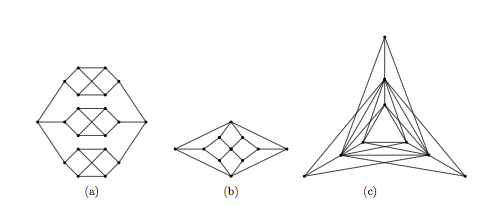
\includegraphics[keepaspectratio]{1.png}\\
	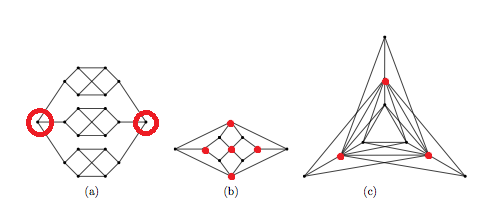
\includegraphics{1_sol.png}\\
	\begin{enumerate}
	\item Удалим вершины, обведенные в красный круг. Очевидно, что останется граф, в котором три компоненты связности. А удаляли мы две вершины. Необходимое условие не выполняется, значит гамильтонова цикла нет.
	\item Удалим красные вершины. Очевидно, что остается граф, состоящий из шести висячих вершин, то есть граф, в котором 6 компонент связности. А удалили мы 5 вершин. Необходимое условие не выполняется, значит гамильтонова цикла нет.
	\item Удалим красные вершины. Очевидно, что остается граф, состоящий из трех висячих вершин и полного графа на три вершины (в центре), то есть граф, в котором 4 компоненты связности. А удалили мы 3 вершины. Необходимое условие не выполняется, значит гамильтонова цикла нет.
	\end{enumerate}
	\item[3.12.] \textit{Доказать, что в графе Петерсена гамильтонова цикла нет.}\\
	Назовем ребра, составляющие внешний пентагон - внешними ребрами, ребра, составляющие внутреннюю пентаграмму - внутренними. Остальные ребра - мостами (не путать с мостом - ребром, удаление которого влечет увеличение числа компонент связности).\\
	Предположим, гамильтонов цикл там есть. Так как это цикл, то он должен вернуться в исходную вершину, а значит должен проходить четное число раз по мостам - 2 или 4.
	\begin{enumerate}
	\item Предположим, в цикле ровно 2 моста. Тогда их концы, как в пентаноне, так и в пентаграмме, должны быть соединены путями длины 4 (так как длина гамильтонова цикла есть 10). Тогда эти концы должны быть смежными как в пентагоне, так и в пентаграмме, что невозможно (это легко проверить).
	\item Предположим, в цикле ровно 4 моста. Рассмотрим пару вершин, являющиеся концами невыбранного моста: в графе должны быть ребра, инцидентные этим двум вершинам, чтобы можно было до них добраться и выбраться. В итоге, мы уже выбрали 8 (4 моста и по 2 ребра на каждый конец неиспользуемого моста) из 10 ребер возможного цикла. Легко понять, что какие бы мы два ребра не добавили -- никакого гамильтонова цикла не будет.\\
	Можно еще заметить, что в таком случае на внешнем и внутреннем цикле должно быть по 3 ребра (они выделены синим), включая пару для концов неиспользуемого моста (на рисунке этот мост -- красный). Такой граф только один -- но он состоит из двух циклов длины 5, причем они лежат в разных компонентах связности (это необходимо, чтобы не образовалось "листьев": вершин степени 1)\\
	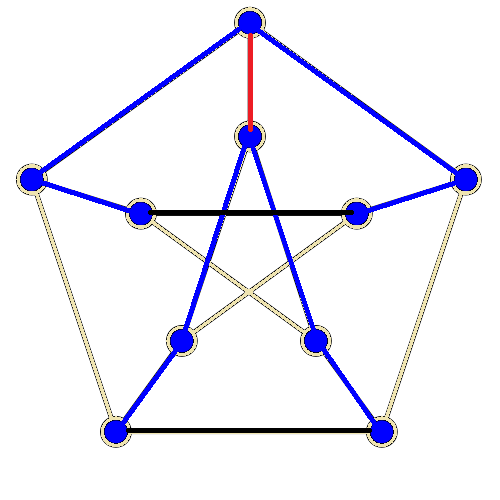
\includegraphics[scale=0.5]{petersen_ham.png}\\
	\end{enumerate}
	\item[3.13.] \textit{Возможно ли удалить в графе Петерсена ребра так, чтобы в полученном графе $G$ существовал эйлеров цикл?}\\
	\begin{enumerate}
	\item Так как граф Петерсена состоит из "двух" циклов, можно удалить все ребра, принадлежащие внутренней пентаграмме и удалить ребра между внутренней пентаграммой и внешним пентагоном - после удаления висячих вершин получится граф $C_5$ (циклический граф на 5 вершин) - в нем очевидно есть эйлеров цикл.
	\item Можно привести еще более сильный пример: в графе Петерсена нельзя удалить ребра так, чтобы он оставался связным и в нем существовал бы эйлеров цикл.\\
	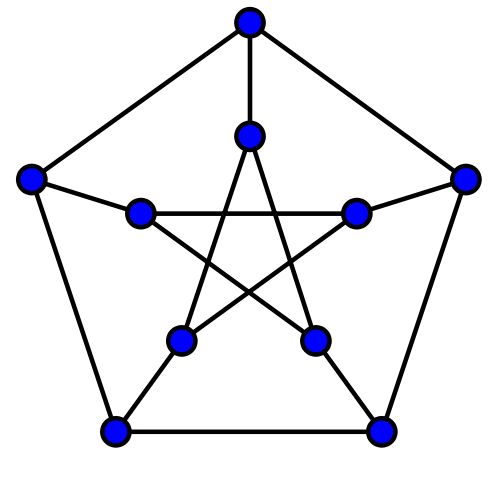
\includegraphics[scale=0.4]{petersen.png}\\
	Назовем ребра, составляющие внешний пентагон - внешними ребрами, ребра, составляющие внутреннюю пентаграмму - внутренними. Остальные ребра - мостами (не путать с мостом - ребром, удаление которого влечет увеличение числа компонент связности).\\
	Отметим, что если в нашем графе существует эйлеров цикл, то в нем степени всех вершин равны двум. (вообще-то они должны быть четными, но мы можем лишь удалять ребра, а поэтому, степени могут только уменьшаться: а так как в графе Петерсона у всех вершин степень 3, то в "эйлеровом" графе у всех вершин должны быть степени 2). Значит, по лемме о рукопожатиях, в этом графе должно быть $2*10/2 = 10$ ребер.\\
	Очевидно, что хотя бы одно из внешних ребер должно быть удалено (в противном случае у всех вершин на пентагоне степень станет УЖЕ равной двум, что повлечет обязательное удаление всех мостов - а значит граф станет несвязным)\\
	В силу симметрии мы можем удалить любое внешнее ребро (отмечено красным). Синим отмечены ребра, которые обязаны быть в графе (чтобы степени соответствующих вершин были равны двум):
	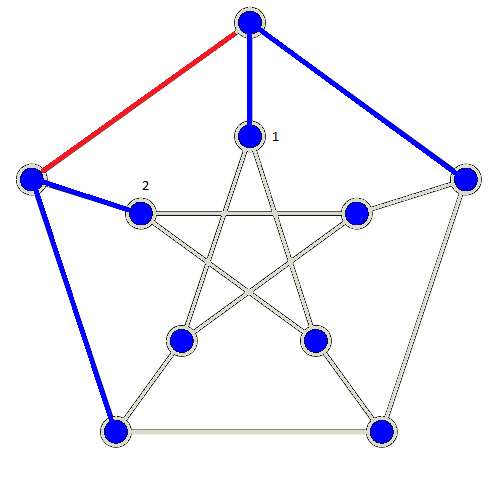
\includegraphics[scale=0.5]{petersen_1.png}\\
	Отметим, что в силу симметрии, мы можем удалить любое еще не рассмотренное ребро, выходящее из вершин 1 или 2 (причем и вершину можем выбрать любую):\\
	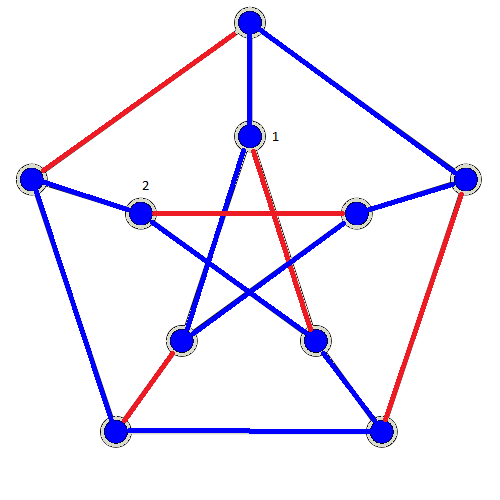
\includegraphics[scale=0.5]{petersen_2.png}\\
	Затем аналогично отмечаем ребра, которые обязаны быть в графе в силу его регулярности. Легко заметить, что больше свободы выбора у нас нет - помечание ребра красным сразу влечет еще два синих (обязательных) ребра и так далее.\\
	Видим, что получился несвязный граф. Значит, в силу симметрии, связного эйлерова графа, полученного из графа Петерсона удалением ребер, не существует.
	\end{enumerate}
	\item[3.14.] \textit{Доказать теорему Хватала.}\\
	\newtheorem*{th1}{Теорема Хватала}
	\begin{th1}
	Пусть $G$ есть простой граф построенный на $n > 2$ вершинах. Рассмотрим упорядоченную по неубыванию последовательность $(d_1,\ldots,d_n)$ степеней $d_k:=deg(x_k)$ вершин графа $G$. Будем называть ее просто "последовательность степеней". Предположим, что не существует индекса $k < n/2$, для которого одновременно выполняются неравенства $d_k \leqslant k$ и $d_{n-k} < (n-k)$. Тогда в $G$ существует гамильтонов цикл.
	\end{th1}
	\begin{proof}
	Докажем сначала 100500 лемм
	
	\newtheorem*{lemma0}{Лемма об условии}
	\begin{lemma0}
	Условие эквивалентно требованию истинности импликации
	\[\forall k \in \mathbb N : (d_k \leq k < n/2 \rightarrow d_{n - k} \geq n - k)\]
	\end{lemma0}
	\begin{proof} 	
	Становится очевидным после небольшого разбора случаев. Не существует индекса, для которого выполняются сразу 2 условия означает, что для любого индекса ложно либо первое, либо второе, либо оба сразу. А это эквивалентно истинности импликации, где второе неравенство обращено (импликация ложна только когда посылка истинна, а заключение ложно).
	\qedhere
	\end{proof}
	
	\newtheorem*{lemma1}{Лемма о добавлении ребра в граф}
	\begin{lemma1}
	Пусть граф $G'$ получен из графа $G$ добавлением нового ребра $e$. Тогда последовательность степеней графа $G'$ мажорирует последовательность степеней графа $G$.
	\end{lemma1}
	\begin{proof}
	
	\newtheorem*{lemma1_1}{Подлемма}
	\begin{lemma1_1}
	Если в неубывающей последовательности $(d_1,\ldots,d_n)$ увеличить на единицу число $d_i$, а затем привести последовательность к неубывающему виду (поставив число $d_i+1$ на свое место $j$), то новая полученная последовательность будет мажорировать исходную.
	\end{lemma1_1}
	\begin{proof}
	Если число никуда двигать не нужно, то есть $j=i$, то утверждение подлеммы, очевидно, выполняется. Пусть $j \neq i$
	\begin{itemize}
	\item Рассмотрим элементы с номерами $s = \overline{1, i - 1}$: они не изменились, следовательно мажорируются собой
	\item Рассмотрим элементы с номерами $s = \overline{i, j - 1}$: они сдвинулись направо, то есть $s$-ый номер полученной последовательности равен $s+1$-ому исходной, поэтому исходные элементы мажорируются элементами новой последовательности.
	\item Рассмотрим элементы с номером $j$: $d'_j \geqslant d'_{j-1}=d_j$
	\item Рассмотрим элементы с номерами $s = \overline{j+1, n}$: они не изменились, следовательно мажорируются собой
	\end{itemize} \qedhere
	\end{proof}	
	При добавлении ребра в граф степени ровно двух вершин увеличиваются на единицу: поэтому для доказательстав леммы просто дважды применим утверждение подлеммы. \\\qedhere
	\end{proof}
	
	\newtheorem*{lemma2}{Лемма о левой части}
	\begin{lemma2}
	$d_k \leq k \Leftrightarrow |\{ v \in V(G) | d_v \leq k \}| \geq k.$
	\end{lemma2}
	\begin{proof} 	
	\begin{enumerate}
	\item
	Необходимость ($\Rightarrow$).\\
	Имеем:
	\begin{itemize}
	\item $d_1 \leq d_2 \leq \ldots \leq d_k$
	\item $d_k \leq k$
	\item $|\{ d_1, d_2, \ldots, d_k \}| = k$
	\end{itemize}
	Тогда: $\{ d_1, d_2, \ldots, d_k \} \subseteq \{ v \in VG | d_v \leq k \} \Rightarrow |\{ v \in V(G) | d_v \leq k \}| \geq k$
	
	\item
	Достаточность ($\Leftarrow$).\\
	Имеем:
	\begin{itemize}
	\item $|\{ v \in VG | d_v \leq k \}| = k + p$
	\item $p \geq 0$
	\end{itemize}
	Расположим вершины в неубывающем порядке их степеней.\\
	Тогда: $d_1 \leq d_2 \leq \ldots \leq d_k \leq \ldots \leq d_{k + p} \leq k \Rightarrow d_k \leq k$
	\end{enumerate}
	\qedhere
	\end{proof}	
	
	\newtheorem*{lemma3}{Лемма о правой части}
	\begin{lemma3}
	$d_{n - k} \geq n - k \Leftrightarrow |\{ v \in V(G) | d_v \geq n - k \}| \geq k + 1.$
	\end{lemma3}
	\begin{proof} 	
	\begin{enumerate}
	\item
	Необходимость ($\Rightarrow$).\\
	Имеем:
	\begin{itemize}
	\item $d_{n - k} \geq n - k$
	\item $d_{n - k} \leq d_{n - k + 1} \leq \ldots \leq d_n$
	\item $|\{ d_{n - k}, d_{n - k + 1}, \ldots , d_n \}| = k + 1$
	\end{itemize}
	Тогда: $\{ d_{n - k}, d_{n - k + 1}, \ldots , d_n \} \subseteq \{ v \in VG | d_v \geq n - k \} \Rightarrow \{ v \in V(G) | d_v \geq n - k \} \geq k + 1$
	
	\item
	Достаточность ($\Leftarrow$).\\
	Имеем:
	\begin{itemize}
	\item $|\{ v \in VG | d_v \geq n - k \}| = k + 1 + p$
	\item $p \geq 0$
	\end{itemize}
	Расположим вершины в невозрастающем порядке их степеней.\\
	Тогда: $d_n \geq d_{n - 1} \ldots \geq d_{n - k} \geq \ldots \geq d_{n - k - p} \geq n - k \Rightarrow d_{n - k} \geq n - k$
	\end{enumerate}
	\qedhere
	\end{proof}
	
	\newtheorem*{lemma4}{Лемма о действии расширения графа на импликацию}
	\begin{lemma4}
	Если импликация (в первой лемме) верна для некоторой последовательности степеней $d$, то она остается верной и для неубывающей последовательности $d'$, мажорирующей $d$. 
	\end{lemma4}
	\begin{proof} Разберем случаи: \\
	\begin{itemize}
	\item Пусть $d'_k > k$. Тогда посылка импликации ложна, следовательно импликация верна вне зависимости от заключения.
	\item Пусть $d'_k \leq k, \mbox{ } d'_{n - k} \geq d_{n - k} \geq n - k$. Тогда и посылка и заключение импликации истинны.
	\end{itemize}
	Значит, импликация, истинная для некоторой последовательности степеней, истинна и для мажорирующей последовательности. \qedhere
	\end{proof}
	
	Леммы закончились, можно доказывать теорему. \textbf{От противного.}\\
	Пусть существует граф с числом вершин не меньше трех, для которого выполняются условия импликации, но в котором нет гамильтонова цикла. Будем добавлять в него ребра до тех пор, пока не получим максимально возможный граф $G$, в котором нет гамильтонова цикла. По лемме о добавлении ребра в граф и лемме о действии расширения графа на импликацию, импликация остается верной для графа $G$.\\
	Выберем две несмежные вершины $u$ и $v$ графа $G$, такие что $\deg u + \deg v$ максимально. Будем считать, что $\deg u \leq \deg v$. Добавив к $G$ новое ребро $e = (u,v)$, получим гамильтонов граф $G + e$. Рассмотрим гамильтонов цикл графа $G + e$: в нём обязательно присутствует ребро $e$. Отбрасывая ребро $e$, получим гамильтонову $(u, v)$-цепь в графе $G$: $u = u_1 \rightarrow u_2 \rightarrow \ldots \rightarrow u_n = v$.\\
	Пусть $S = \{ i | e_i = u_1 u_{i + 1} \in E(G)\}, T = \{ i |f_i = u_i u_n \in E(G)\}$. Пересечение этих двух подмножеств пусто: действительно, пусть $j \in S \cap T$, тогда $u_1 \rightarrow u_{j + 1} \rightarrow \ldots \rightarrow u_n \rightarrow u_j \rightarrow u_{j - 1} \rightarrow \ldots \rightarrow u_1$ - гамильтонов цикл, противоречие.\\
	Из определений $S$ и $T$ следует, что $S \cup T \subseteq \{1, 2, ..., n - 1 \} \Rightarrow 2 \deg u \leq \deg u + \deg v = |S| + |T| = |S \cup T| < n$. Значит, $\deg u < n/2$.\\
	Так как $S \cap T  = \emptyset$, ни одна вершина $ u_j $ не смежна с $ v = u_n $ (для $ j \in S $). В силу выбора $ u $ и $ v $, получим, что $ \deg u_j \leq \deg u $. Пусть $ k = \deg u = |S| $. Значит, $ \exists k $ вершин, степень которых не превосходит $k$.\\
	По лемме о левой части: $d_k \leq k < n/2$. В силу импликации: $ d_{n - k} \geq n - k$.\\
	По лемме о правой части: $\exists k + 1$ вершин, степень которых не меньше $n - k$.\\
	Так как $ k = \deg u $, то вершина $u$ может быть смежна максимум с $k$ из этих $k+1$ вершин. Значит, существует вершина $w$, не являющаяся смежной с $u$ и для которой $ \deg w \geq n - k $. Тогда получим, что $ \deg u + \deg w \geq k + (n - k) = n > \deg u + \deg v $, что противоречит тому, что вершины $u$ и $v$ выбраны так, что их суммарная степень максильмана.\\
	Получили противоречие. Теорема доказана.			
	\end{proof}
\end{enumerate}
\end{document}
